\documentclass[journal]{vgtc}                % final (journal style)
%\documentclass[review,journal]{vgtc}         % review (journal style)
%\documentclass[widereview]{vgtc}             % wide-spaced review
%\documentclass[preprint,journal]{vgtc}       % preprint (journal style)
%\documentclass[electronic,journal]{vgtc}     % electronic version, journal

%% Uncomment one of the lines above depending on where your paper is
%% in the conference process. ``review'' and ``widereview'' are for review
%% submission, ``preprint'' is for pre-publication, and the final version
%% doesn't use a specific qualifier. Further, ``electronic'' includes
%% hyperreferences for more convenient online viewing.

%% Please use one of the ``review'' options in combination with the
%% assigned online id (see below) ONLY if your paper uses a double blind
%% review process. Some conferences, like IEEE Vis and InfoVis, have NOT
%% in the past.

%% Please note that the use of figures other than the optional teaser is not permitted on the first page
%% of the journal version.  Figures should begin on the second page and be
%% in CMYK or Grey scale format, otherwise, colour shifting may occur
%% during the printing process.  Papers submitted with figures other than the optional teaser on the
%% first page will be refused.

%% These three lines bring in essential packages: ``mathptmx'' for Type 1
%% typefaces, ``graphicx'' for inclusion of EPS figures. and ``times''
%% for proper handling of the times font family.

\usepackage{mathptmx}
\usepackage{graphicx}
\usepackage{times}
\usepackage{balance}
\usepackage[nooneline,hang,it,IT]{subfigure}

%% We encourage the use of mathptmx for consistent usage of times font
%% throughout the proceedings. However, if you encounter conflicts
%% with other math-related packages, you may want to disable it.

%% This turns references into clickable hyperlinks.
\usepackage[bookmarks,backref=true,linkcolor=black]{hyperref} %,colorlinks
\hypersetup{
  pdfauthor = {},
  pdftitle = {},
  pdfsubject = {},
  pdfkeywords = {},
  colorlinks=true,
  linkcolor= black,
  citecolor= black,
  pageanchor=true,
  urlcolor = black,
  plainpages = false,
  linktocpage
}

%% If you are submitting a paper to a conference for review with a double
%% blind reviewing process, please replace the value ``0'' below with your
%% OnlineID. Otherwise, you may safely leave it at ``0''.
\onlineid{0}

%% declare the category of your paper, only shown in review mode
\vgtccategory{Research}

%% allow for this line if you want the electronic option to work properly
\vgtcinsertpkg

%% In preprint mode you may define your own headline.
%\preprinttext{To appear in an IEEE VGTC sponsored conference.}

%% Paper title.

\title{\LARGE TN1008 \\ Advanced Simulation and Visualization of Fluids in Computer Graphics \\ \Large Divergence-Free Smoothed Particle Hydrodynamics}

%% This is how authors are specified in the journal style

%% indicate IEEE Member or Student Member in form indicated below
\author{Ronja Grosz, rongr946\\ Isabell Jansson, isaja187\\ Jonathan Bosson, jonbo665}
\date{\today}
%\authorfooter{
%% insert punctuation at end of each item
%\item
 %Ronja Grosz is a student at Link\"oping University, Sweden, e-mail: rongr946@student.liu.se.
%}

%% Abstract section.
\abstract{ 
}
%% Keywords that describe your work. Will show as 'Index Terms' in journal
%% please capitalize first letter and insert punctuation after last keyword
\keywords{Divergence-free, SPH, divergence correction, density correction.}



%%%%%%%%%%%%%%%%%%%%%%%%%%%%%%%%%%%%%%%%%%%%%%%%%%%%%%%%%%%%%%%%
%%%%%%%%%%%%%%%%%%%%%% START OF THE PAPER %%%%%%%%%%%%%%%%%%%%%%
%%%%%%%%%%%%%%%%%%%%%%%%%%%%%%%%%%%%%%%%%%%%%%%%%%%%%%%%%%%%%%%%%

\begin{document}

\firstsection{Introduction}
\maketitle 
    %explain the context of the work:
	%What exactly is the problem?
	%What have you created?
    Smoothed particle hydrodynamics, \textit{SPH}, is a method that was first implemented in 1977 for astrophysical simulations by Gingold et al.~\cite{firstSPH}.
    Since then SPH has become a popular method for complex water simulations.
    SPH is a mesh-free Lagrangian method where the particles move in space and change physical properties as time progresses.
    % More about Lagrangian and maybe navier stokes?
    
    % We used this article
    In this paper we are going to introduce the results from reproducing the divergence-free smoothed particle hydrodynamics method introduced by Bender et al.~\cite{bender}.
    It is a method which corrects the divergence error, aiming for a divergence-free velocity field which is needed for an incompressible fluid.
    For the solution to be divergence-free the density has to be constant over time.
    
    % Write about other solutions? Why is this solution the BEST!!?

\section{Background and Related Work}
    %What have people done before?
	%When addressing this problem, when addressing similar problems
    %What have you done that makes you approach different?

    % Bridson
    ~\cite{bridson}.

    % Write about Benders article


\section{Method}
%What have you done?
%How did you do it?
%Why did you do it that way?
%May want to mention why you *didn’t* do it in some 
%other possible way
%Clear enough that you could hand the report to another student and they could reproduce the work!
%Probably no need to mention programming language etc
\subsection{Neighbourhood search}
    Since SPH only considers a finite amount of neighbouring particles, it is important to keep track of every particles neighbours.
    Searching through all particles for neighbours within the cutoff distance $H$ for every particle is inefficient and takes $\mathcal{O}({N^2})$ time.
    The cutoff distance $H$ is the kernel smoothing radius.
    To fasten this up a cell list was implemented.
    A cell list is a data structure that is divided into cells that have a length larger or equals to the cutoff distance $H$.
    When finding the neighbour of particle $i$, only the neighbouring cells have to be searched for particles within the cutoff distance, see figure~\ref{fig:cellList}.
    
    \begin{figure}
    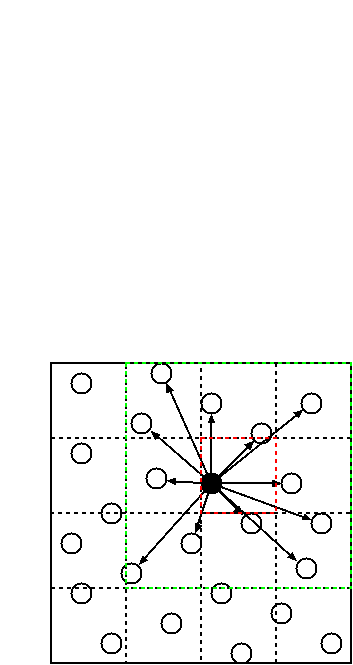
\includegraphics[width=\linewidth]{img/CellLists2.png}
    \caption{Finding the neighbours for the filled in particle $i$ by looking through all neighbouring cells, including its own cell, for particles within the cutoff distance $H$}
    \label{fig:cellList}
    \end{figure}

    The cell list is implemented by using a four dimensional vector where the first three dimensions are for the x, y and z coordinates for the cells and the fourth dimension is for storing the particles belonging to the cell.
    The amount of cells are decided by dividing the scene into cells of length $H$.
    The particles are then assigned to a cell according to equation~ref{eq:assignCell}.
    If the particle moves out of its cell it is then assigned to the new cell.

    \begin{equation} \label{eq:assignCell}
        sjdfkljsf
    \end{equation}


\subsection{Divergence solver}
\subsection{Density solver}
\subsection{Kernel}
\subsection{Navier-stokes}
% Write about non pressure forces, velocity osv..?
\subsection{Adapted time step}
\subsection{Density and alpha factors}
\subsection{Screen space fluid rendering}

\section{Implementation}
%Details of how it was done
%What hardware
%What software
%Why did you do it that way?
%What limitations, if any, did this present?
%*No code*!!!!!
 
    % Talk about what we used for plugins, computers etc maybe or should this be in method?

\section{Results}
%What is the end product:
%What does it look like?
%How does one control and interact with it?
%How quick is it?
%What limitations does it have?
%Be self-critical and honest about it - or I will be



\section{Conclusions and Future Work}
%Based on the results and evaluation
%Say what you’ve done right... ...and what you’ve done wrong! - be honest!
%Suggest some possible ways that the work could have been done better
%Suggest some ways that it could be extended and improved by adding more effort

% Use ghost-SPH or similar

%\bibliographystyle{abbrv}
\bibliographystyle{ieeetr}
\bibliography{./refs}

\end{document}
\grid
